\documentclass{article}

\usepackage{geometry}
\usepackage{gbt7714}
\usepackage{xeCJK}
\usepackage{booktabs}       % professional-quality tables
\usepackage{amsfonts}       % blackboard math symbols
\usepackage{subfig}
\usepackage{amsmath}
\usepackage{graphicx}
\usepackage{float}
\usepackage{svg}

\graphicspath{{assets/}}


\linespread{1.5}
\geometry{a4paper, left=2.5cm, right=2.5cm, top=2.5cm, bottom=2.5cm}
\bibliographystyle{gbt7714-numerical}   
\title{基于潜在正则化对抗的特高压直流换流阀声音异常检测}

\begin{document}
\maketitle

\begin{abstract}

换流阀是高压直流输电系统的核心组件，负责交流电与直流电之间的转换，确保电能高效、稳定地长距离输送和分配。然而，实际系统中的故障发生频率较低且种类多样，导致全面收集异常样本具有较大挑战性。有监督的检测方法依赖大量标记的正常和异常数据进行训练，而传统的基于重构或对抗学习的异常检测方法在潜在空间中难以分离正常数据和异常数据，无法实现高效的检测效果。
针对这些问题，本文提出了一种新的无监督异常检测方法，即潜在变量正则化对抗异常检测方法（Latent Regularization Adversarial Anomaly Detection, LRAAD）。LRAAD的训练方式与生成对抗网络类似，但是LRAAD使用编码器来充当判别器的作用。生成对抗网络的判别器将输入的频谱图映射到一个标量值，表示输入图像是真实数据的概率。而编码器在LRAAD模型中的判别任务是更加复杂的，它将输入的频谱图映射到潜在空间，并通过潜在表示与标准正态分布的KL散度来判别输入频谱图的真实性。这种判别方式使得编码器学习到输入频谱图的关键特征，并将其映射到潜在空间，使得生成器能够生成更加符合真实数据分布的样本。
本文在换流站实测声音数据集上进行了实验验证，结果显示LRAAD方法在异常检测任务上的AUC指标和p-AUC指标明显优于其他基线模型，验证了该方法的有效性和实用性，为异常声音检测在换流阀状态监测领域提供了新的解决方案。

\end{abstract}


关键字：异常声音检测, 无监督学习, 对抗学习, 潜在变量正则化对抗

\section{引言}
随着电力系统的不断发展和升级，特高压输电技术在全球范围内得到了广泛应用。特高压换流站作为电力系统的重要组成部分，其运行状态直接关系到电力输送的可靠性和稳定性。然而，换流阀等关键设备在运行过程中可能会出现局部放电等异常情况，导致系统性能下降甚至引发严重故障。为了确保电力系统的安全运行，准确、高效的异常检测方法显得尤为重要。传统的换流阀异常检测方法主要依赖于振动、温度等物理参数的监测，而基于声音信号的检测方法逐渐受到重视\cite{AR-AD}。

在异常检测中，异常数据通常难以获得，因为实际系统中的故障发生频率较低且种类多样，导致收集全面的异常样本具有较大挑战性。有监督的检测方法依赖大量标记的正常和异常数据进行训练，但由于异常数据稀缺，这些方法在实际应用中表现出局限性，难以应对未见过的异常情况。

传统的异常检测方法主要依赖于手动检查和简单的统计分析，无法应对复杂多变的工况，且对实际应用中的实时性要求难以满足。近年来，基于机器学习和深度学习的异常检测方法逐渐兴起，显示出较高的检测精度和良好的适应性。然而，现有的基于重构或对抗学习的异常检测方法在潜在空间中难以有效分离正常数据和异常数据，限制了其实际应用效果。

针对上述问题，本文提出了一种新的无监督异常检测方法——潜在变量正则化对抗的异常检测方法（Latent Regularization Adversarial Anomaly Detection, LRAAD）。该方法在潜在空间域进行对抗学习，利用编码器充当判别器的角色，使得正常数据的潜在表示与标准正态分布的KL散度最小化，即打高分，而生成数据的潜在表示与标准正态分布的KL散度最大化，即打低分，从而实现了编码器能够对正常数据和异常数据进行有效判别。

LRAAD模型包括两个主要模块：编码器和生成器。编码器接收输入的频谱图并将其转换为潜在空间的表示，同时通过最小化正常数据的潜在表示与标准正态分布的KL散度，优化潜在空间的分布。生成器则负责将潜在变量映射回频谱图域，生成尽可能真实的频谱图，通过对抗学习不断提高生成器的生成能力。编码器与生成器的联合训练，使得模型能够在不同负载条件下有效检测异常。

实验中采用的数据集来源于中国某±800kV特高压换流站的换流阀实测声音数据。根据换流阀运行时的视在功率不同，数据集被划分为六个子集，分别对应400MVA到1000MVA的视在功率范围。这些数据不仅包括正常运行状态下的声音，还包含局部放电等故障时的声音特征，为模型的训练和验证提供了丰富的样本。

本文的主要贡献包括以下几点：

\begin{enumerate}

  \item 提出了一种新的异常检测方法LRAAD，通过潜在空间域的对抗学习，实现正常数据和异常数据的有效分离。

  \item 使用特高压换流站的实测声音数据对模型进行了验证，实验结果表明，LRAAD方法在不同负载条件下均表现出较高的异常检测准确率和鲁棒性。

\end{enumerate}

本文的结构安排如下：第二章介绍了相关研究工作和背景知识；第三章详细描述了LRAAD模型的设计和实现，包括编码器和生成器的架构及其训练方法；第四章介绍了实验设置和数据集划分，并对实验结果进行分析和讨论；第五章总结了本文的研究工作，并提出了未来的研究方向。

\section{相关工作}

自2020年以来，DCASE任务2\cite{DCASE2020Task2,DCASE2021Task2,DCASE2022Task2,DCASE2023Task2}旨在开发一种基于深度学习\cite{DeepLearning-1,DeepLearning-2,DeepLearning-3}的自监督机器异常声音检测模型，以实现对工业设备状态的实时监控和故障预警。最近，许多基于深度学习的自监督异常声音检测方法被开发出来，主要包括基于自编码器的方法\cite{AE-AD,AE-AD-2,CAE-AD,VAE-AD,VAE-AD-2,SAE-AD}、基于流模型的异常检测方法\cite{NF-AD,DifferNet,CFlow-AD}、基于生产对抗网络的异常检测方法\cite{AnoGAN,EGBAD,f-AnoGAN,GANomaly,AEGAN-AD}以及基于自回归网络的异常检测方法\cite{AR-AD,WaveNet-AD}。

\subsection{基于自编码器的异常检测方法}

自编码器（Autoencoder, AE）是一种常用于无监督学习的神经网络结构，广泛应用于异常检测领域。自编码器通过训练一个神经网络将输入数据压缩到低维的潜在空间，然后再通过解码器将其还原到原始维度。自编码器的目标是使重构误差最小化，即输入数据与重构数据之间的差异尽可能小。基于自编码器的异常检测方法利用这一特性，通过分析重构误差来识别异常数据。

在基于自编码器的异常检测方法研究中，研究者们主要关注基于传统的自编码器（AE）\cite{AE-AD}和基于变分自编码器（VAE）\cite{VAE,VAE-AD}的方法。例如，Sabokrou等人\cite{AE-AD}提出了一种基于自编码器的异常检测方法，该方法通过训练一个自编码器来学习正常数据的特征表示，然后使用重构误差来识别异常数据。类似地，Huang等人\cite{AE-AD-2}提出了一种基于AE的视觉异常检测（VAD）方法。该方法首先引入自动编码变压器（AT），以扩大正常样本和异常样本之间的异常分数差距，然后使用AE模型学习正常样本的高层语义特征，从而获得正常样本的潜在表示。Duman等人\cite{CAE-AD}提出了一种基于卷积自编码器（CAE）的异常检测方法，该方法通过训练一个CAE模型来学习正常数据的特征表示，然后使用重构误差来识别异常数据。这些方法在异常检测任务中取得了一定的效果，但是由于自编码器的限制，这些方法在学习复杂的数据分布时表现不佳，导致重构误差较大，模型难以准确拟合。

基于变分自编码器（VAE）的异常检测方法\cite{VAE-AD,VAE-AD-2}通过引入潜在变量和KL散度来学习数据的潜在表示，从而提高模型的泛化能力。例如，An等人\cite{VAE-AD}提出了一种基于变分自编码器的异常检测方法，该方法通过训练一个VAE模型来学习正常数据的潜在表示，然后使用KL散度来衡量正常数据和异常数据之间的差异。


基于自编码器的方法在检测稳定的声音信号方面表现出色，但是由于设备运行工况的多样性，实际的声音信号存在较大的变化，这些方法在学习良好的特征概率分布时表现不佳，导致重构误差较大，模型难以准确拟合\cite{DeepLearning-4}。

\subsection{基于生成对抗网络的异常检测方法}

生成对抗网络（Generative Adversarial Networks, GANs）\cite{GAN}是由Ian Goodfellow等人在2014年提出的一种强大的生成模型，通过两个相互竞争的神经网络（生成器和判别器）对抗训练，实现数据的生成和特征学习。基于GAN的异常检测方法利用GAN的生成能力和判别器的区分能力，通过生成器生成数据并使用判别器来识别异常样本，成为近年来异常检测领域的重要方法之一\cite{GAN-BASED-AD-REVIEW}。

基于GAN的异常检测方法利用GAN的生成能力，通过分析生成数据与实际数据之间的差异来识别异常样本。Schlegl等人提出的AnoGAN\cite{AnoGAN}方法通过GAN的生成器学习正常数据的分布，并利用生成数据与实际数据的差异来检测异常样本，但是该方法需要在推断阶段学习图像到潜在空间的映射，计算耗时。针对这一问题，Schlegl等人\cite{f-AnoGAN}在AnoGAN的基础上进行改进，提出了f-AnoGAN方法，AnoGAN 使用迭代方法寻找图像在潜在空间的表示，f-AnoGAN 通过学习从 图像到潜在空间的映射，显著提高了检测速度。Akcay等人\cite{GANomaly}]提出了一种名为GANomaly 的新型编码器-解码器-编码器架构模型，其同时使用重构损失、潜在表示损失和对抗损失来训练模型和进行异常分数计算，实验表明，其性能优于当代最先进的基于GAN 和传统自编码器的异常检测方法。Jiang等人\cite{AEGAN-AD}提出了一种利用生成对抗网络 （GAN）进行机器音频异常检测的无监督模型AEGAN-AD。研究表明，通过引入鉴别器来提供特征级别 的指导，AEGAN-AD 模型可以更深入地理解表示，而不仅仅关注表面噪音，解决了编码器可能会重构出 异常信号的问题。

\subsection{基于流模型的异常检测方法}

流模型（Flow-based Models）是一类近年来兴起的生成模型，它们通过可逆的变换将复杂的数据分布映射到简单的分布（通常是高斯分布），并且这种变换是可计算其雅可比行列式的，从而能够精确地计算数据的概率密度。流模型在异常检测领域中表现出色，因为它们能够直接估计输入数据的概率密度，进而根据概率密度值来判断数据是否为异常。

近年来，基于流模型的异常检测方法也得到了广泛的研究。例如，Rudolph等人\cite{DifferNet}提出了一种名为DifferNet的半监督缺陷检测方法，采用多尺度特征提取器来处理图像的高维性,使归一化流能够分配有意义的似然度。Gudovskiy等人\cite{CFlow-AD}提出了一种实时无监督异常检测模型CFLOW-AD，利用条件正规化流进行异常定位。Rudolph等人\cite{CSFlow}提出了一种新颖的全卷积跨尺度归一化流（CS-Flow）用于基于图像的缺陷检测。该方法通过联合处理多尺度特征图，模拟无缺陷图像数据的分布，实现了高效的图像异常检测。

流模型的优势在于其高精度的概率估计能力，能够在高维空间中精确建模数据分布。此外，流模型的可逆性保证了无损的数据变换，使其在生成和重构任务中具有很好的性能。在异常检测中，流模型能够准确区分正常数据和异常数据，提高检测的准确率和可靠性。然而，流模型也存在一些挑战和局限性。首先，流模型的训练过程通常需要大量计算资源和时间，尤其是在处理高维数据时。其次，流模型对模型结构和参数设置要求较高，可能需要大量实验调整超参数。此外，流模型在处理离散数据和稀疏数据时，效果可能不如连续数据和密集数据。


\subsection{基于自回归网络的异常检测方法}

自回归模型（Autoregressive Model, AR）是一种统计模型，它使用序列自身的历史值来预测当前或未来的值。自回归模型在时间序列分析中广泛应用，通过建模数据序列中的依赖关系来进行预测。基于自回归模型的异常检测方法利用这种序列依赖性来识别数据中的异常点，特别适用于时间序列数据的异常检测。

基于自回归模型的异常检测方法主要集中在WaveNet模型\cite{WaveNet-AD,AR-AD}。Rushe等人\cite{AR-AD}提出了将WaveNet架构应用于音频异常检测的方法，并通过实验比较了该方法与基准自编码器模型的性能，结果显示WaveNet在几乎所有情况下表现更优。该论文的重要性在于扩展了WaveNet架构的应用领域，并展示了其在音频异常检测方面的有效性。Hayashi等人\cite{WaveNet-AD}提出了一种基于WaveNet的异常声音事件检测方法。该方法利用WaveNet作为一个基于卷积神经网络的生成模型，用于在公共空间中建模各种声学模式。当模型检测到未知声学模式时，将其识别为异常声音事件。


\section{特高压换流阀的声音产生机理及故障声音分析}

特高压换流阀作为电力系统中至关重要的设备，其运行状态直接影响整个系统的可靠性和稳定性。在运行过程中，换流阀会产生多种声音，这些声音不仅反映了设备的正常工作状态，也可能揭示潜在的故障隐患。理解换流阀声音的产生机理及故障声音特征，对于异常检测和故障诊断具有重要意义。

\subsection{换流阀声音产生机理}

换流阀在其运行过程中会产生多种声音，这些声音主要来源于以下几个方面：

\textbf{电磁噪声}是换流阀运行中最常见的声音之一。换流阀内的大量电力电子元件（如晶闸管、IGBT等）在高频开关过程中会产生电磁噪声。这些噪声由电磁波在周围介质中的传播和元件间的电磁相互作用引起，频率较高且音量不大。电磁噪声通常表现为高频的“嗡嗡”声，持续且均匀。

\textbf{机械振动}也是换流阀声音的重要来源。换流阀的开关动作会导致其内部结构部件的机械振动，尤其是在电流突变时，电动力作用会使换流阀的结构件（如冷却系统、支撑架等）发生微小的机械位移，从而发出振动噪声。这类噪声通常频率较低，但振幅较大，表现为低频的“嗡嗡”声或“咚咚”声。

\textbf{冷却系统噪声}也是换流阀运行中不可忽视的部分。为了确保在高负荷运行时的温度控制，换流阀通常配备复杂的冷却系统（如风冷、液冷等）。冷却系统中的风机、泵等设备在运行时会产生明显的噪声，这部分噪声相对稳定，但随着换流阀负载的变化，其音量和频率也会有所不同，通常表现为稳定的“隆隆”声或“呼呼”声。

\textbf{局部放电噪声}是换流阀在高压环境下可能发生的一种特殊声音。局部放电是一种电气故障现象，通常伴随有高频的放电噪声。局部放电噪声由电离过程中的电流脉冲产生，频率范围较广且具有随机性，通常表现为不连续的高频“噼啪”声。

\subsection{换流阀故障声音分析}

不同故障状态下，换流阀会产生特定的声音特征，识别这些声音特征对于异常检测和故障诊断具有重要意义。以下是几种常见故障及其对应的声音特征：

\textbf{局部放电故障}是高压换流阀常见的故障类型之一。局部放电会产生高频的尖锐噪声，类似于“噼啪”声。这种声音通常是不连续的，频率较高（几千赫兹到几十千赫兹），具有明显的随机性和瞬时性。局部放电故障的主要原因包括绝缘材料老化、受潮、局部破损等，这些因素导致局部电场增强，使介质局部电离并产生放电现象。

\textbf{机械故障}会导致换流阀内机械部件的异常振动，发出低频的振动噪声，类似于“嗡嗡”声。这种声音往往是持续的，且音量可能随负载变化而变化。机械故障的原因可能包括固定部件松动、机械磨损、冷却系统故障等，这些问题会导致机械部件振动异常，从而产生明显的低频噪声。

\textbf{冷却系统故障}也会引起特定的声音变化。冷却系统故障会导致风机或泵的运行异常，产生持续的、较大的噪声，类似于“隆隆”声。冷却系统故障的原因可能包括冷却液流动受阻、风机叶片损坏、泵运行不正常等，这些问题会导致冷却系统运行异常，从而产生显著的噪声变化。

\textbf{电磁干扰故障}可能导致高频噪声的增加，表现为持续的高频“滋滋”声。这种声音的频率较高且较稳定，通常伴随着电气设备的开关动作频繁出现。电磁干扰故障的原因可能包括电力电子元件开关频率异常、接触不良等，这些问题会导致电磁干扰增加，从而产生高频噪声。

\section{提出的方法}

生成对抗网络（GAN）\cite{GAN}由Goodfellow等人于2014年提出，是一种通过对抗训练的方式来学习数据分布的生成模型。生成对抗网络由两个神经网络组成：生成器（Generator）和判别器（Discriminator）。判别器的目标是尽可能准确地判断输入数据是真实数据还是生成数据，而生成器的目标是尽可能生成判别器无法区分来源的数据。这两个目标不同的网络不断地进行交替训练，当最后收敛时，生成器可以生成与真实数据分布相似的数据。

LRAAD的训练方式与生成对抗网络类似，但是LRAAD使用编码器来充当判别器的作用。生成对抗网络的判别器将输入的频谱图映射到一个标量值，表示输入图像是真实数据的概率。而编码器在LRAAD模型中的判别任务是更加复杂的，它将输入的频谱图映射到潜在空间，并通过潜在表示与标准正态分布的KL散度来判别输入频谱图的真实性。这种判别方式使得编码器学习到输入频谱图的关键特征，并将其映射到潜在空间，使得生成器能够生成更加符合真实数据分布的样本。


\subsection{模型架构设计}


\subsubsection{编码器}

LRAAD的编码器充当判别器的作用。不同于生成对抗网络的判别器，生成对抗网络的判别器将输入的频谱图映射到一个标量值，表示输入图像是真实数据的概率。而编码器在LRAAD模型中的判别任务是更加复杂的，它需要将输入的频谱图映射到潜在空间，并通过潜在表示与标准正态分布的KL散度来判别输入频谱图的真实性。这种判别任务需要编码器学习到输入频谱图的关键特征，并将其映射到潜在空间，以便后续的生成器能够生成尽可能真实的频谱图。

\begin{figure}[h]
    \centering
    
\includegraphics[width=0.45\textwidth]{./assets/encoder.pdf}
    \caption{The architecture of the encoder $E$}
    \label{fig:encoder}
\end{figure}

编码器的最后一层输出不同于常规的全连接层，如图\ref{fig:encoder}所示。它采用的是均值和方差参数来表示潜在空间的分布，这是基于变分自编码器（Variational Autoencoder，VAE）的思想。通过这种设计，编码器不仅可以生成潜在表示，还能够学习到潜在空间的分布信息，使得潜在表示可以与标准正态分布进行比较。这种比较主要通过KL散度来衡量，KL散度小表示潜在表示接近标准正态分布，反之则表示潜在表示与标准正态分布的分布差异较大。潜在变量$z$的KL散度的计算公式如下：

\begin{equation}
    D_{KL}(q(z|x)||p(z)) = \frac{1}{2} \sum_{i=1}^{N}(\sigma_i^2 + \mu_i^2 - \log(\sigma_i^2) - 1)
\end{equation}

编码器在训练过程中，通过最小化正常数据的潜在表示与标准正态分布之间的KL散度，来学习将正常数据映射到接近标准正态分布的潜在空间。与此同时，学习将异常数据(生成器生成的数据)的潜在表示映射到偏离标准正态分布的潜在空间区域。这种训练方式使得编码器能够更好地区分正常数据和异常数据，因为正常数据在潜在空间中更加紧密地分布，而异常数据则会显著地偏离标准正态分布。

\subsubsection{生成器}

生成器的结构与解码器类似。生成器的输入是编码器生成的潜在变量$z$，输出是生成的频谱图。生成器的目标是通过学习将潜在变量映射到与正常数据频谱图相似的图像，从而提供优质的正常数据样本来优化编码器的学习过程。生成器的训练与编码器交替进行，利用对抗学习的框架来不断提高生成器的生成能力。

\begin{figure}[H]
    \centering
    \def\svgwidth{\textwidth}
    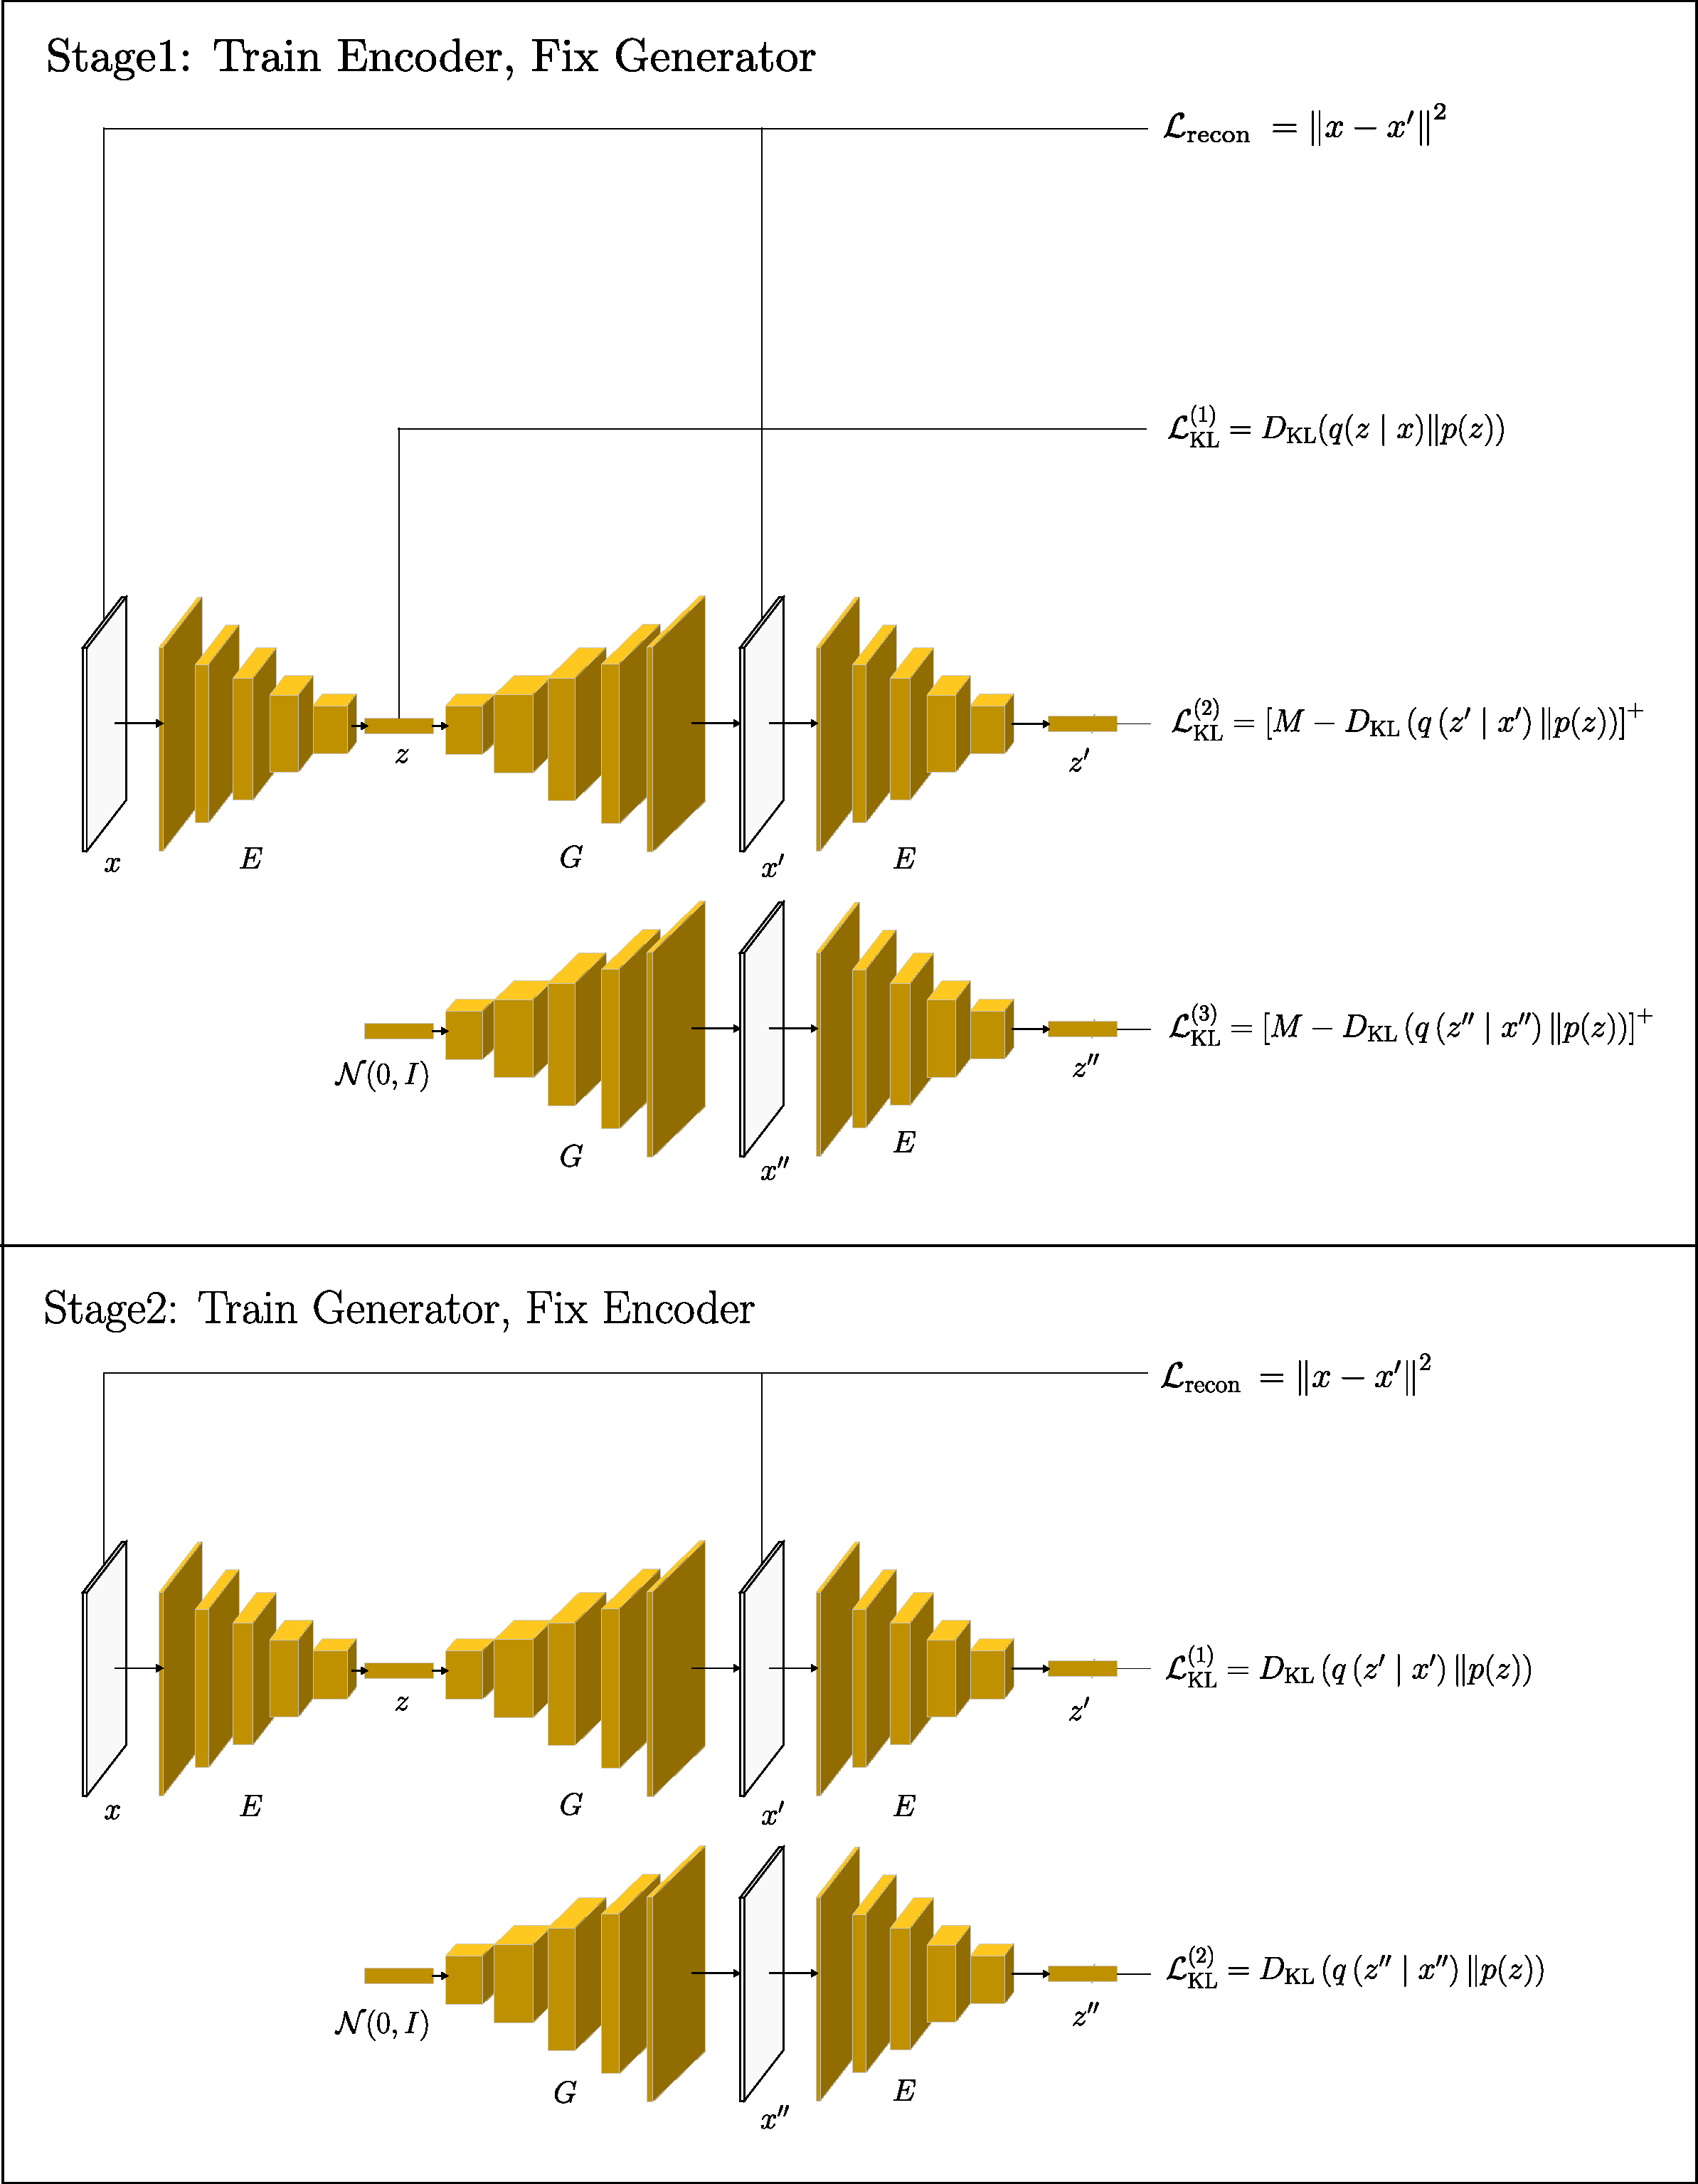
\includegraphics[width=\textwidth]{./assets/lraad_model.pdf}
    \caption{The Training Pipeline of LRAAD}
    \label{fig:lraad}
\end{figure}

\subsection{模型训练}
首先，LRAAD的流程以编码器开始。编码器接收一张频谱图（通常是梅尔频谱图）作为输入，并将其转换为潜在空间的表示。这个表示是对输入频谱图的抽象表达，记为$z$。编码器的目标是通过学习将正常数据的潜在表示尽可能接近标准正态分布，而将异常数据的潜在表示远离标准正态分布。这样的训练过程可以使得编码器能够更好地区分正常和异常数据。

接下来是生成器的训练阶段。生成器接收编码器生成的潜在变量 z，并将其映射回频谱图的梅尔频谱域，生成尽可能真实的频谱图。生成器的目标是通过学习将潜在变量映射到与正常数据频谱图相似的图像，从而提供优质的正常数据样本来优化编码器的学习过程。生成器的训练与编码器交替进行，利用对抗学习的框架来不断提高生成器的生成能力。

下面详细介绍LRAAD模型的训练过程及其损失函数设计。

\subsubsection{编码器训练}

编码器的训练目标是将正常数据的潜在表示$z$尽可能接近标准正态分布，同时将生成数据的潜在表示$z^\prime$和$z^{\prime\prime}$远离标准正态分布。为了实现这一目标，编码器需要学习如何在潜在空间中对输入频谱图进行有效的表示。通过对抗学习的方式，编码器不断优化其输出，使得正常数据和异常数据在潜在空间中实现分离。编码器的训练损失主要包括KL散度损失和重构损失两部分。

\textbf{KL散度损失：} KL散度损失用于衡量编码器生成的潜在表示 z 与标准正态分布的差异。在LRAAD模型中，KL散度损失通过计算潜在表示的分布与标准正态分布$p(z)=\mathcal{N}(0, I)$之间的KL散度来评估它们的相似性。对于正常数据，编码器的目标是最小化其KL散度损失，使其潜在表示与标准正态分布尽可能接近。对于生成数据，编码器的目标是最大化其KL散度损失，使其潜在表示远离标准正态分布。这样的训练方式可以促使编码器将正常数据和异常数据在潜在空间中分离开来，从而使得编码器可以充当判别器的角色，有效区分正常数据和异常数据。

\begin{equation}
  \mathcal{L}_{\mathrm{KL}}=D_{\mathrm{KL}}(q(z \mid x) \| p(z)) + [M - D_{\mathrm{KL}}\left(q\left(z^{\prime} \mid x^{\prime}\right) \| p(z)\right)]^{+} + [M - D_{\mathrm{KL}}\left(q\left(z^{\prime \prime} \mid x^{\prime \prime}\right) \| p(z)\right)]^{+}
\end{equation}

其中，$q(z \mid x)$表示编码器编码正常数据$x$的潜在表示的分布，$q(z^\prime \mid x^\prime)$和$q(z^{\prime\prime} \mid x^{\prime\prime})$分别表示编码器编码生成数据$x^\prime$和$x^{\prime\prime}$的潜在表示的分布。$p(z)$表示标准正态分布，记为$\mathcal{N}(0, I)$。$D_{\mathrm{KL}}$表示KL散度，$[M - D_{\mathrm{KL}}]^{+}$表示KL散度的修正项，其中$M$是一个超参数，用于控制KL散度的上限。

\textbf{重构损失：}重构损失衡量的是输入数据与重建数据之间的差异。在LRAAD模型中，重构损失用于确保编码器生成的潜在表示 z 能够准确地重建原始输入频谱图 x。具体来说，编码器生成潜在表示$z$后，通过生成器将$z$反向映射回频谱图域，生成重建的频谱图$x^\prime$。重构损失的目标是最小化$x$与$x^\prime$之间的差异，常用的重构损失函数是均方误差（Mean Squared Error，MSE）, 其计算公式如下：

\begin{equation}
\mathcal{L}_{\text {recon }}=\left\|x-x^{\prime}\right\|^2
\end{equation}

总的损失函数为：

\begin{equation} \label{eq:encoder_loss}
  \mathcal{L_E}=\beta_{\text {KL }} \cdot\mathcal{L}_{\text {KL }}+\beta_{\text {recon }} \cdot\mathcal{L}_{\text {recon }}
\end{equation}

\subsubsection{生成器训练}
生成器的目标与判别器相反，即让判别器将自己生成的样本判别为真实样本。生成器的训练过程始于接收编码器编码正常数据$x$生成的潜在变量$z$和在正态分布中采样的潜在变量$z_{p}$。生成器将潜在变量$z$和$z_{p}$作为输入，并通过一系列神经网络层，逐步将其反向映射到频谱图的梅尔频谱域，生成频谱图$x^\prime$和$x^{\prime \prime}$。生成器的目标是生成的频谱图$x^\prime$和$x^{\prime \prime}$能够尽可能真实地接近正常数据的频谱图。在训练过程中，生成器和编码器通过对抗学习的框架相互优化，使得生成器不断提高生成频谱图的质量，同时优化编码器的判别能力。生成器的训练损失主要包括对抗性损失和重构损失两部分。

\textbf{对抗性损失：}对抗性损失用于衡量生成器生成的频谱图$x^\prime$和$x^{\prime \prime}$与正常数据频谱图之间的差异。在LRAAD模型中，对抗性损失通过判别器$D$来评估生成器生成的频谱图的真实性。判别器的目标是区分正常数据频谱图和生成的频谱图，使得生成器生成的频谱图更加真实。对抗性损失的计算公式如下：

\begin{equation}
  \mathcal{L}_{\text {adv }}=D_\mathrm{KL}(q(z^\prime \mid x^\prime) \| p(z)) + D_\mathrm{KL}(q(z^{\prime\prime} \mid x^{\prime\prime}) \| p(z))
\end{equation}

\textbf{重构损失：}重构损失用于衡量生成的频谱图 x' 与真实输入频谱图 x 之间的差异。这一损失确保生成器能够准确地还原输入频谱图的特征。重构损失通常采用均方误差（MSE）来计算：

\begin{equation} \label{eq:generator_loss}
  \mathcal{L}_{\text {recon }}=\left\|x-x^{\prime}\right\|^2
\end{equation}

总的损失函数为：

\begin{equation}
  \mathcal{L_G}=\beta_{\text {adv }} \cdot\mathcal{L}_{\text {adv }}+\beta_{\text {recon }} \cdot\mathcal{L}_{\text {recon }}
\end{equation}

LRAAD模型的训练过程如表\ref{tab:training}所示。在训练过程中，编码器和生成器通过对抗学习的方式相互优化，使得编码器能够学习到正常数据的潜在表示，并将其映射到标准正态分布，同时将异常数据的潜在表示映射到偏离标准正态分布的区域。生成器的目标是生成尽可能真实的频谱图，使得编码器能够更好地区分正常数据和异常数据。通过这种方式，LRAAD模型能够有效地拟合正常数据的分布。


\begin{table}[H]
    \centering
    \begin{tabular}{l}
        \toprule
        \label{tab:training}
        {\textbf{Algorithm} Training LRAAD model} \\
        \midrule
        1: Initialize network parameters \\
        2: \quad {\textbf{For} number of epochs \textbf{do}} \\
        3: \quad\quad Random mini-batch $X$ from dataset \\
        4: \quad\quad Compute latent representation of $X$: $Z = E(X)$ \\
        5: \quad\quad Sample $Z_p$ from prior distribution $p(z)=\mathcal{N}(0, I)$ \\
        6: \quad\quad Compute reconstructed spectrogram of $Z$ and $Z_p$: $X^\prime = G(Z)$, $X^{\prime\prime} = G(Z_p)$ \\
        7: \quad\quad Compute latent representation of $X^\prime$ and $X^{\prime\prime}$: $Z^\prime = E(X^\prime)$, $Z^{\prime\prime} = E(X^{\prime\prime})$ \\
        8: \quad\quad Compute Encoder loss $\mathcal{L}_E$ according to Eq. \ref{eq:encoder_loss} \\
        9: \quad\quad Update Encoder parameters by minimizing $\mathcal{L}_E$ \\
        10: \quad\quad Compute Generator loss $\mathcal{L}_G$ according to Eq. \ref{eq:generator_loss} \\
        11: \quad\quad Update Generator parameters by minimizing $\mathcal{L}_G$ \\
        12: \quad {\textbf{End For}} \\


        \bottomrule
    \end{tabular}
\end{table}


\subsection{异常检测}

在训练完成后，我们可以使用训练好的生成器和编码器来计算每个输入频谱图的异常分数。异常分数用于衡量输入频谱图与正常数据分布之间的差异，从而识别出潜在的异常。

我们使用重构误差作为异常分数来衡量输入数据与模型生成数据之间的差异，从而识别潜在的异常。具体地，对于给定的梅尔频谱图输入$x$，我们首先通过编码器将其映射到潜在空间中得到潜在变量$z$。然后，使用生成器从潜在变量$z$生成重构的频谱图$x^\prime$。重构的频谱图$x^\prime$与原始输入$x$的L1误差作为异常分数。其计算公式如下：

\begin{equation}
\mathcal{A}(x)=\left\|x-G\left(E(x)\right)\right\|_1
\end{equation}
其中，$\mathcal{A}(x)$是输入梅尔频谱图$x$的异常分数，$E(x)$是编码器$E$的输出的潜在变量，$G(E(x))$是生成器$G$从潜在变量生成的重构频谱图。重构误差越大，表示重构的频谱图与原始输入之间的差异越大，可能表明输入的频谱图具有异常或不正常的特征。

在实际应用中，我们可以设置一个阈值来判断重构误差是否超过正常范围，并将超过阈值的样本标记为异常。通过这种方式，我们可以使用重构误差作为异常分数来进行声学异常检测，从而识别出潜在的异常或不正常的电力设备声学信号。

% \section{实验：Experiments}
\section{Experiments}
本节我们将介绍实验的设置和结果。我们首先介绍实验的数据集和预处理方法，然后详细描述实验的设置和评估指标，最后给出实验结果和分析。

\subsection{Dataset}
本实验采用的数据集是从中国某\(\pm\)800kV特高压换流站的换流阀实测声音数据。这些数据是通过在换流站安装的传声器实时采集得到的，用于监测换流阀在运行过程中产生的声音信号。这些数据包含了换流站在正常运行状态下以及可能存在异常情况下记录的声音信号。在正常运行状态下，换流站产生的声音信号应当是稳定的，并且不会出现异常噪音。而在异常情况下，可能会出现各种故障或异常情况，例如设备摩擦、松动、电弧放电等，这些异常情况可能会导致声音信号的突变或异常增加。因此，通过分析和识别声音信号中的异常模式，可以帮助监测和诊断换流站设备的健康状况。

该数据集包含了一系列声音信号的录音文件，录音文件以 WAV 格式存储，每个文件记录了在不同时间点下换流站产生的声音信号。每个录音文件的采样频率为44.1Hz，持续时间为10秒。在数据集的收集过程中，我们尽可能涵盖了换流站设备可能遇到的各种正常和异常情况，以确保数据集的多样性和代表性。同时，我们还对录音文件进行了标注，将正常状态和异常状态的声音信号区分开来，以便于实验和分析。


换流阀的视在功率范围为400MVA到1000MVA，根据视在功率的不同，将实测声音数据分为六个子集，分别记为Dataset1至Dataset6。每个数据集对应一个特定的视在功率范围，具体如下：

\begin{table}[h!]
\centering
\begin{tabular}{c c}
\toprule
\textbf{数据集} & \textbf{视在功率范围 (MVA)} \\
\midrule
Dataset1 & 400 - 500 \\
Dataset2 & 500 - 600 \\
Dataset3 & 600 - 700 \\
Dataset4 & 700 - 800 \\
Dataset5 & 800 - 900 \\
Dataset6 & 900 - 1000 \\
\bottomrule
\end{tabular}
\caption{视在功率范围对应的数据集}
\label{table:datasets}
\end{table}


为了进行实验，我们将每个录音文件切分为多个长度为1.36秒的音频片段，然后将每个音频片段转换为对应的梅尔频谱图。梅尔频谱图是声音信号的一种常用表示形式，它可以更好地反映声音信号的频谱特征。我们使用梅尔频谱图作为模型的输入，以便于模型学习和分析声音信号的频谱特征。对于每个梅尔频谱图，我们对其进行对数变换和归一化处理，以便于模型训练和优化。

\subsection{Data Preprocessing}

在进行声学信号的异常检测实验时，数据预处理是非常关键的一步，它直接影响到后续模型的训练和异常检测的准确性。下面是我们对实验数据进行的详细预处理步骤：


为了更好地处理数据和提取特征，我们首先将长时间的音频信号分段为较短的片段。这可以通过滑动窗口的方式进行，每个窗口包含一段时间内的音频数据。这样做的目的是使得数据更易于处理，并且可以更精确地捕获声音的时间特征。


对于每个音频分段，我们使用梅尔频率倒谱系数（Mel Frequency Cepstral Coefficients，MFCC）来表示其频谱特征。梅尔频谱是在横坐标上使用Mel刻度，纵坐标上是功率谱的一种表示方式，更符合人类听觉感知的特性。我们使用Librosa等库来进行梅尔频谱转换，将每个音频分段转换为对应的梅尔频谱图。 对于得到的梅尔频谱图，我们对其进行对数变换。这一步骤可以有效地增强低频特征的信息，减少高频特征的干扰，使得数据更加平滑和稳定。

接下来，我们对经过对数变换的梅尔频谱图进行归一化处理。归一化的目的是将数据缩放到一个统一的范围内，以避免不同特征之间的数值差异对模型训练造成影响。我们使用最小-最大归一化来处理数据。

\subsection{Experimental Settings}

LRAAD 模型包含编码器、生成器和判别器三个主要部分。编码器使用了由 CAE 提出的架构，包括五个卷积层，负责将输入的梅尔频谱图映射到潜在空间中的均值和方差。生成器则采用了 DCGAN 提出的架构，包括五个反卷积层，用于将潜在变量映射回梅尔频谱域，实现频谱图的重建。判别器也采用了 DCGAN 的架构，包括五个卷积层，用于判断输入的频谱图是真实数据还是生成数据。这种架构的设计旨在平衡编码器的特征提取能力、生成器的重建能力和判别器的区分能力，从而提高异常检测的准确性和鲁棒性。

在训练 LRAAD 模型时，我们需要设置多个超参数来调节模型的性能。例如，编码器和生成器的学习率、损失函数的权重系数（如重构损失、对抗损失、KL 散度损失的权重）、潜在空间的维度大小、训练的迭代次数等。这些超参数的选择对模型的训练和性能具有重要影响，需要通过实验和验证来确定最佳的超参数组合。在实验中，我们采用的超参数设置如Table \ref{tab:params}所示：


\begin{table}[htbp]
    \centering
    \caption{LRAAD Model Hyperparameter Settings}
    \label{tab:params}
    \begin{tabular}{lr}
        \toprule
        \textbf{Hyperparameter} & \textbf{Setting} \\
        \midrule
        Latent Space Dimension & 32 \\
        Learning Rate (Encoder) & 0.0002 \\
        Learning Rate (Generator) & 0.0002 \\
        Loss Weight (Reconstruction) & 1 \\
        Loss Weight (Adversarial) & 1 \\
        Loss Weight (KL Divergence) & 1 \\
        M (KL Divergence Limit) & 100 \\
        Training Epochs & 100 \\
        Batch Size & 32 \\
        Dataset Split & 80\% Training, 30\% Testing \\
        \bottomrule
    \end{tabular}
\end{table}


% \subsection{评估指标：Evaluation Metrics}
\subsection{Evaluation Metrics}
在实验中，评估指标是对模型性能进行客观量化和比较的重要标准。我们主要使用了AUC（Area Under the ROC Curve）和p-AUC（Partial Area Under the ROC Curve）这两个常用的评估指标来评估异常检测模型的效果。

ROC曲线（Receiver Operating Characteristic Curve）：ROC曲线是用于评估二分类模型性能的图形工具，横轴表示假阳性率（False Positive Rate，FPR），纵轴表示真阳性率（True Positive Rate，TPR）。ROC曲线能够直观展示在不同阈值下模型的真阳性率与假阳性率之间的权衡关系。一般来说，ROC曲线越接近左上角（TPR高、FPR低），说明模型性能越好，对异常检测问题来说，ROC曲线的面积（AUC）越大，表示模型对于正常和异常样本的区分能力越强。

AUC（Area Under Curve）：AUC是ROC曲线下方的面积，用于衡量模型分类效果的一个总体指标。AUC的取值范围在0.5到1之间，其中0.5表示模型性能等同于随机分类，1表示完美分类。在异常检测任务中，AUC值越接近1，说明模型对正常和异常样本的区分能力越强，具有更好的检测准确度。

p-AUC（Partial Area Under Curve）：p-AUC是ROC曲线的局部面积，用于评估模型在低假阳性率（FPR）下的性能。在异常检测任务中，p-AUC值越大，表示模型在低FPR下的检测性能越好，能够更准确地识别出异常样本。

ROC 曲线和 AUC 指标是评估异常检测模型性能的重要指标，能够直观地反映模型在识别异常样本和正常样本方面的表现，并帮助比较不同模型的性能优劣。

% \subsection{实验结果：Experimental Results}
\subsection{Experimental Results}
为验证LRAAD模型在异常检测领域的检测性能，本实验将LRAAD模型与CAE、AnoGAN、GANomaly等经典异常检测模型进行了对比实验。实验结果表明，LRAAD模型在异常检测任务上取得了更好的性能表现，具有更高的AUC和p-AUC值，能够更准确地识别出异常样本。

Figure \ref{fig:roc_curve}展示了LRAAD模型与其他模型在异常检测任务上的ROC曲线比较。从图中可以看出，LRAAD模型的ROC曲线处于其他模型的上方，AUC值更高，表明LRAAD模型具有更好的性能表现。表\ref{tab:auc}、表\ref{tab:p-auc-03}、表\ref{tab:p-auc-02}和表\ref{tab:p-auc-01}分别展示了不同模型在不同数据集上的AUC和p-AUC值的比较。从表中可以看出，LRAAD模型在所有数据集上均取得了更高的AUC和p-AUC值，相比其他模型具有更好的异常检测性能。

\begin{table}[H]
    \centering
    \begin{tabular}{cccccc}
        \toprule
        Dataset & CAE & VAE & f-AnoGAN & GANomaly & LRAAD(Our) \\
        \midrule
        Dataset1 & 0.8975 & 0.8662 & 0.8400 & 0.8966 & \textbf{0.9361} \\
        Dataset2 & 0.8911 & 0.8652 & 0.8560 & 0.9195 & \textbf{0.9475} \\
        Dataset3 & 0.9266 & 0.8958 & 0.8662 & 0.9266 & \textbf{0.9607} \\
        Dataset4 & 0.9087 & 0.8868 & 0.8654 & 0.9333 & \textbf{0.9626} \\
        Dataset5 & 0.8962 & 0.8965 & 0.8910 & 0.9511 & \textbf{0.9721} \\
        Dataset6 & 0.8523 & 0.8178 & 0.8126 & 0.8270 & \textbf{0.8674} \\
        \bottomrule
    \end{tabular}
    \caption{AUC Comparison of Different Models on Different Datasets}
    \label{tab:auc}
\end{table}


\begin{table}[H]
    \centering
    \begin{tabular}{cccccc}
        \toprule
        Dataset & CAE & VAE & f-AnoGAN & GANomaly & LRAAD(Our) \\
        \midrule
        Dataset1 & 0.6664 & 0.5824 & 0.5161 & 0.7232 & \textbf{0.7930} \\
        Dataset2 & 0.6394 & 0.5559 & 0.5487 & 0.7843 & \textbf{0.8430} \\
        Dataset3 & 0.7605 & 0.6576 & 0.5935 & 0.8076 & \textbf{0.8639} \\
        Dataset4 & 0.6972 & 0.6252 & 0.5790 & 0.8164 & \textbf{0.8342} \\
        Dataset5 & 0.6529 & 0.6569 & 0.6423 & 0.8705 & \textbf{0.8866} \\
        Dataset6 & 0.5262 & 0.4656 & 0.4589 & 0.5243 & \textbf{0.6335} \\
        \bottomrule
    \end{tabular}
    \caption{p-AUC Comparison of Different Models on Different Datasets (FPR<0.3)}
    \label{tab:p-auc-03}
\end{table}

\begin{table}[H]
    \centering
    \begin{tabular}{cccccc}
        \toprule
        Dataset & CAE & VAE & f-AnoGAN & GANomaly & LRAAD(Our) \\
        \midrule
        Dataset1 & 0.5431 & 0.4503 & 0.3809 & 0.6417 & \textbf{0.7078} \\
        Dataset2 & 0.5355 & 0.4192 & 0.4037 & 0.7324 & \textbf{0.7865} \\
        Dataset3 & 0.7041 & 0.5225 & 0.4598 & 0.7496 & \textbf{0.8176} \\
        Dataset4 & 0.6142 & 0.5014 & 0.4532 & 0.7609 & \textbf{0.8173} \\
        Dataset5 & 0.5465 & 0.5390 & 0.5371 & \textbf{0.8332} & 0.8115 \\
        Dataset6 & 0.3801 & 0.3190 & 0.3227 & 0.3935 & \textbf{0.5377} \\

        \bottomrule
    \end{tabular}
    \caption{p-AUC Comparison of Different Models on Different Datasets (FPR<0.2)}
    \label{tab:p-auc-02}
\end{table}

\begin{table}[H]
    \centering
    \begin{tabular}{cccccc}
        \toprule
        Dataset & CAE & VAE & f-AnoGAN & GANomaly & LRAAD(Our) \\
        \midrule
        Dataset1 & 0.3640 & 0.2736 & 0.2261 & 0.5268 & \textbf{0.5629} \\
        Dataset2 & 0.4405 & 0.2472 & 0.2318 & 0.6353 & \textbf{0.6658} \\
        Dataset3 & 0.6024 & 0.3372 & 0.2651 & 0.6810 & \textbf{0.7020} \\
        Dataset4 & 0.5487 & 0.3345 & 0.3136 & 0.6635 & \textbf{0.6993} \\
        Dataset5 & 0.4090 & 0.3700 & 0.3964 & \textbf{0.7626} & 0.7400 \\
        Dataset6 & 0.2168 & 0.1566 & 0.1624 & 0.2330 & \textbf{0.3791}\\

        \bottomrule
    \end{tabular}
    \caption{p-AUC Comparison of Different Models on Different Datasets (FPR<0.1)}
    \label{tab:p-auc-01}
\end{table}

\begin{figure}
  \centering
  \includegraphics[width=0.45\linewidth]{./experiments/ssva1/roc_curve.pdf}
  \hfill
  \includegraphics[width=0.45\linewidth]{./experiments/ssva2/roc_curve.pdf}
  \hfill
  \includegraphics[width=0.45\linewidth]{./experiments/ssva3/roc_curve.pdf}
  \hfill
  \includegraphics[width=0.45\linewidth]{./experiments/ssva4/roc_curve.pdf}
  \hfill
  \includegraphics[width=0.45\linewidth]{./experiments/ssva5/roc_curve.pdf}
  \hfill
  \includegraphics[width=0.45\linewidth]{./experiments/ssva6/roc_curve.pdf}
  \caption{ROC Curves of Different Models on Different Datasets}
\end{figure}

\section{Conclusion}
 LRAAD模型通过引入编码器和生成器两个模块，实现了在潜在空间中的对抗学习，并使用编码器作为判别器，使正常数据的潜在表示与标准正态分布的KL散度最小化，而生成数据的潜在表示与标准正态分布的KL散度最大化，从而实现了编码器对正常数据和异常数据在潜在空间中的有效分离。

 LRAAD模型在AUC指标和p-AUC指标上都实现了较高的性能，这表明模型具有较好的异常声音检测能力，可以有效地区分正常声音和异常声音，有助于及时发现换流阀的潜在问题和故障。通过与其他经典模型如CAE、VAE、f-AnoGAN和GANomaly的对比实验，LRAAD模型在异常检测领域的表现明显优于其他模型，这验证了模型的有效性和实用性。LRAAD模型通过引入潜在变量正则化对抗学习，提高了模型对异常声音的敏感性和识别能力，从而更好地适应实际工业生产中的异常检测任务。

 但是，仍有一些需要改进和深入探讨的地方,具体如下:第一，可以探索更多的损失函数组合和优化策略，以提高模型的鲁棒性和泛化能力。第二,论文没有对模型各部分超参数的敏感性进行分析。对模型各部分超参数的敏感性分析,有助于把握模型行为，能让我们更好地理解不同超参数对模型表现的影响,从而指导参数调优,获得最佳性能。第三,异常分数计算的方式较为简单,或许可以探索更复杂的异常分数度量方式。当前的异常分数仅利用了重建误差,将来可以考虑引入其他先验知识,设计更合理的异常分数函数。第四,可以进一步分析LRAAD在不同类型异常声音上的表现,看看是否存在一些模式偏好。对于复杂的工业场景,不同类型的异常可能需要专门的建模方式,了解当前模型的偏好有助于指导下一步改进方向。第四,模型的可解释性有待加强,这对异常检测任务很重要。高可解释性能让异常结果更易被人类理解和判断,从而提高异常检测系统的可信赖性。

\bibliography{references}

\end{document}

